%-----------------------------------------------------------------------------%
\chapter{\babDua}
%-----------------------------------------------------------------------------%


%-----------------------------------------------------------------------------%
\section{Definisi Pengawakan}
%-----------------------------------------------------------------------------%

Menurut Rivai dan Segala (2010:198) :
\\
“Kepuasan kerja akan tercapai bila terdapatnya kesesuaian karyawan dengan posisi pekerjaan yang mereka dapatkan. Posisi \textit{staffing} karyawan berarti mengalokasikan para karyawan pada posisi kerja tertentu”\cite{2}.

Kemudian, Ardana (2012:18) menambahkan mengenai posisi \textit{staffing} sebagai berikut : 
\\
“Posisi \textit{staffing} karyawan merupakan pencocokan atau membandingkan kualifikasi yang dimiliki dengan persyaratan pekerjaan dan sekaligus memberikan tugas, pekerjaan kepada calon karyawan untuk dilaksanakan”\cite{2}.

Pengertian diatas dapat disimpulkan bahwa posisi \textit{staffing}  yang tepat tidak cukup. Untuk menunjang kinerja karyawan, melainkan membutuhkan pengalaman kerja karyawan untuk menunjang pekerjaan tersebut.  




%-----------------------------------------------------------------------------%
\section{Proses Pengawakan}
%-----------------------------------------------------------------------------%

Menurut T. Hani Handoko (2000:230) langkah-langkah dalam porses \textit{staffing} meliputi beberapa aspek yaitu \cite{3}: 

\begin{enumerate}

\item Perencanaan sumber daya manusia \\
Pemenuhan kebutuhan organisasi untuk mengisi posisi tertentu, untuk itu perlu adanya perencanaan yang terdiri atas:
\begin{enumerate}
	
\item Penentuan jabatan yang akan diisi, kemampuan yang dibutuhkan, serta jumlah yang dibutuhkan.

\item Pemahaman pasar tenaga kerja potensial.

\item Pertimbangan kondisi permintaan dan penawaran karyawan. Apabila suatu perusahaan membutuhkan tenaga kerja baru, maka perusahaan akan mencari orang yang cakap dan terampil untuk mengisi tugas yang kosong tersebut serta mempunyai motivasi untuk melaksanakan misi dan tujuan perusahaan tersebut. Perusahaan bisa memperoleh tenaga kerja tersebut melalui dua sumber yaitu, sumber dari perusahaan (\textit{intern}) dan sumber dari luar perusahaan (\textit{ekstern}), sumber dari dalam perusahaan yaitu dengan menggunakan orang-orang yang bekerja dalam perusahaan tersebut terutama dalam rangka promosi dan mutasi jabatan, sedangkan sumber yang berasal dari luar perusahaan seperti sekolah-sekolah, departemen tenaga kerja, iklan, dan lain-lain.

\end{enumerate}

\item Penarikan tenaga kerja \\
Rekruitmen karyawan dilakukan untuk menggantikan pekerjaan lama yang telah berhenti dikarenakan pensiun, meninggal, mengundurkan diri atau diberhentikan karena suatu kebijakan tertentu. Pada organisasi \textit{fitness center}, penambahan dan rekruitmen jumlah karyawan atau instruktur juga disesuaikan dengan penambahan jumlah pendaftaran \textit{members} baru.

\item Penyeleksian tenaga kerja \\ 
Seleksi adalah kegiatan untuk mendapatkan tenaga kerja yang paling cakap dan memenuhi persyaratan jabatan. Dalam proses seleksi ini diadakan penilaian sifat-sifat dan karateristik calon pegawai yang diterima, yaitu calon yang memenuhi syarat sebagaimana telah ditentukan. Dalam \textit{requirement} karyawan, terjadi tahapan pengumuman pendaftaran, tahapan pendaftaran sesuai bidang yang dibutuhkan, serangkaian tes atau seleksi, dan pengumuman kelulusan. Para peserta yang lulus seleksi akhir, dinyatakan sebagai karyawan baru yang siap berkontribusi pada organisai. 

\item Kualitas pegawai baru \\
Orientasi pegawai sangat penting terutama bagi perusahaan besar dimana pimpinan tidak mungkin mengadakan pengawasan langsung. Masa percobaan ini merupakan proses penerimaan pegawai dari penerimaan sampai diterimanya pegawai tersebut menjadi pegawai tetap atau secara resmi.

\item Latihan dan pengembangan karyawan \\
Tenaga kerja perlu dilatih dan dikembangkan agar dapat melaksanakan pekerjaannya dengan baik. Manfaat dari latihan dan pengembangan adalah untuk mempermudah seseorang melakukan tugasnya. Dengan adanya latihan dan pengembangan yang baik, perusahaan akan memperoleh tenaga kerja, yang cakap dan terlatih sehingga dapat melakukan pekerjaanya dengan efisien. Dalam melaksanakan tugasnya, seorang karyawan tidak mungkin statis, tetapi harus dinamis serta senantiasa berusaha untuk untuk dapat meningkatkan prestasi dan hasil karyanya, oleh karena itu keterampilan dan pengetahuan karyawan perlu dikembangkan melalui “\textit{in service training}”.

\item Penilaian pelaksanaan kerja karyawan \\
Pada dasarnya penilaian pegawai mempunyai manfaat ganda karena dapat digunakan sebagai alat dalam mengambil keputusan seperti untuk pembayaran upah, gaji, bonus, alat dan pemberian nasehat kepada pegawai. Penilaian sebaiknya dilakukan oleh suatu tim yang terdiri dari atasan langsung sebagai ketua, psikolog, dan seseorang lainnya sebagai anggota. Penilaian karyawan mengacu pada sistem karir dan hasil prestasi kerja. Pada sistem karir yang dilihat adalah kecakapan karyawan yang bersangkutan, pengalaman dalam bekerja, kesetiaan pada organisasi, pengabdian dari segi lamanya waktu bekerja dan syarat objektif lainnya. 

\item Pemberian balas jasa dan penghargaan \\
Kompensasi diberikan sebagai balas jasa dan penghargaan kepada karyawan. Kompensasi yang diberikan perusahaan bisa sebagai alat untuk memotivasi pegawai agar bekerja dengan lebih baik. Kompensasi merupakan kompensasi biaya yang besar bagi perusahaan. Hal ini perlu mendapatkan perhatian agar biaya yang dikeluarkan tidak sia-sia. Pemberian balas jasa ini meliputi pembayaran insentif atau gaji harus adil, layak, tepat waktu sesuai denga peraturan yang berlaku, dan memberikan kepuasan kepada semua pihak baik karyawan maupun atasan atau pimpinan.

\end{enumerate}

Dengan adanya langkah-langkah tersebut, perusahaan berharap dapat memperoleh tenaga kerja yang benar-benar sesuai dengan kebutuhan dan dapat bekerja dengan efisien dan efektif sehingga terjadi peningkatan produktivitas kerja dan sebagai dampak akhirnya perusahaan mencapai tujuannya.

%-----------------------------------------------------------------------------%
\section{Manfaat Pengawakan}
%-----------------------------------------------------------------------------%

Manfaat dari pengawakan terdiri dari:

\begin{enumerate}

\item Memposisikan pegawai sesuai dengan \textit{job description}.

\item Karyawan bekerja dengan baik karena adanya latihan dan pengembangan yang baik.

\item Perusahaan mengalami peningkatan produktivitas kerja sehingga dapat mencapai tujuan dengan efisien.

\end{enumerate}

%-----------------------------------------------------------------------------%
\section{Tujuan Pengawakan}
%-----------------------------------------------------------------------------%

Menurut Janet B. Parks (2007:338) tujuan penyusunan pengawakan adalah \cite{3}:

\begin{enumerate}

\item Terwujudnya sinergitas pekerjaan sesuai dengan seluruh tugas dan kewajibannya.

\item Terwujudnya mekanisme kerja yang koperatif, efektif dan terpadu.

\item Memudahkan pekerjaan dengan keahlian pada bidang masing-masing menyelesaikan tugasnya dengan baik.

\item Mendorong pekerjaan untuk memberikan dana guna dan hasil guna yang maksimal bagi organisasi.

\end{enumerate}

%-----------------------------------------------------------------------------%
\section{Hasil Manajemen Pengawakan}
%-----------------------------------------------------------------------------%

Program manajemen pengawakan yang berhasil dapat membantu perusahaan untuk menjawab tantangan bisnis, memasuki wilayah pasar yang baru dan bergerak maju menyaingi kompetitor. Karyawan yang bertalenta akan lebih tertarik untuk bekerja diperusahaan yang menghargai karyawan dan memberikan kesempatan untuk terus menggapai keberhasilan.

%-----------------------------------------------------------------------------%
\subsection{Manfaat Manajemen Pengawakan}
%-----------------------------------------------------------------------------%

Menurut Pella dan Inayati (2011:87) \cite{4} : \\
“Manfaat program manajemen talenta yaitu tersedia terus-menerus karyawan yang mencapai potensi terbaik mereka masing-masing, maupun mengembangkan reputasi publik untuk menjadi tempat bekerja yang bagus, sekaligus memupuk loyalitas para karyawan yang telah bekerja didalam perusahaan.

\newpage

%-----------------------------------------------------------------------------%
\section{MySQL dan Basis Data}
%-----------------------------------------------------------------------------%

\begin{figure}
	\centering
	
\includegraphics[width=0.4\textwidth]
	{pics/mysql.png}
	\caption{MySQL \textit{Database}}
	\label{fig:31}
\end{figure}

Menurut Wahana Komputer (2010:21) : \\
“MySQL adalah \textit{database server open source} yang cukup popular keberadaannya. Dengan berbagai keunggulan yang dimiliki, membuat \textit{software} database ini banyak digunakan oleh praktisi untuk membangun suatu project.Adanya fasilitas API (\textit{Application Programming Interface} ) yang dimiliki oleh MySQL, memungkinkan bermacam – macam aplikasi komputer yang ditulis dengan berbagai bahasa pemrograman dapat mengakses basis data MySQL.” \\

Tipe data MySQL, menurut Kustiyahningsih (2011:147) : \\
“Tipe data MySQL adalah data yang terdapat dalam sebuah tabel berupa \textit{field – field} yang berisi nilai dari data tersebut. Nilai data dalam \textit{field} memiliki tipe sendiri – sendiri”.

Beberapa keunggulan MySQL dibandingkan dengan database lain adalah \cite{5} :

\begin{enumerate}

\item Kecepatan MySQL cepat \\
Para pengembang berpendapat bahwa MySQL adalah \textit{database} yang tercepat yang didapat. Pendapat ini dapat diselidiki dengan mengunjungi http://www.mysql.com/benchmark.html

\item Kemudahan dalam penggunaan \\
MySQL adalah simple database sistem dengan performa tinggi dan tidak kompleks untuk \textit{set up, administrator}, dibanding dengan sistem yang lebih besar.

\item Mendukung bahasa \textit{Query} \\
MySQL memahami SQL, juga dapat mengakses MySQL menggunakan aplikasi yang mendukung ODBC.

\item Kemampuan banyak \textit{client} dapat berhubungan \textit{server} pada saat yang bersamaan. \textit{Clients} dapat menggunakan \textit{multiple database} secara bersamaa. 

\end{enumerate} 

%-----------------------------------------------------------------------------%
\section{\textit{Framework} Laravel}
%-----------------------------------------------------------------------------%

\begin{figure}
	\centering
	
\includegraphics[width=0.6\textwidth]
	{pics/laravel.png}
	\caption{\textit{Framework} Laravel}
	\label{fig:31}
\end{figure}

Laravel adalah sebuah \textit{framework} web yang berbasis PHP yang tidak berbayar dan \textit{open-source}, diciptakan oleh Taylor Otwell dan diperuntukkan untuk pengembangan aplikasi web yang menggunakan pola MVC (\textit{Model, View, Controller}). Pola MVC memiliki struktur yang berbeda dari struktur pola MVC pada umumnya.

Pengertian \textit{framework} menurut Naista adalah : \\
“Suatu struktur konseptual dasar yang digunakan untuk memecahkan atau menangani suatu masalah yang kompleks. Singkatnya, \textit{framework} adalah wadah atau kerangka kerja dari sebuah \textit{website} yang akan dibangun. Dengan menggunakan kerangka tersebut waktu yang digunakan dalam membuat \textit{website} lebih singkat dan memudahkan dalam melakukan perbaikan.”

“Salah satu \textit{framework} yang banyak digunakan oleh \textit{programmer} adalah \textit{framework} laravel. Laravel adalah \textit{framework} berbasis PHP yang sifatnya \textit{open source}, dan menggunakan konsep \textit{model – view – controller}. Laravel berada di bawah lisesni MIT, License dengan menggunakan Github sebagai tempat berbagi \textit{code} (Naista, 2017).”

“Dalam penggunaanya laravel memiliki beberapa kekurangan salah satunya yaitu ukuran file yang cukup besar. Di dalam laravel terdapat file yang sifatnya default seperti vendor. File tersebut tidak boleh dihapus sembarangan sehingga ukuran website yang dibuta berukuran cukup besar. Selain itu, dibutuhkan koneksi internet untuk instalasi dan mengunduh \textit{library} laravel, dan PHP minimal versi 5.4 untuk menjalankannya (Naista, 2017).” 

\begin{figure}
	\centering
	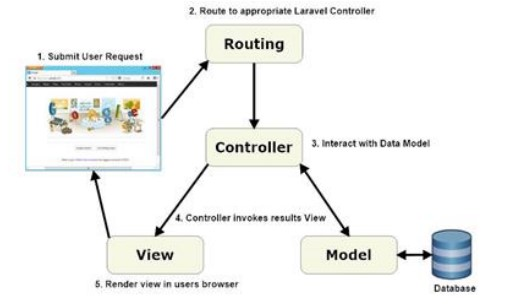
\includegraphics[width=0.7\textwidth]
	{pics/ilustrasimvc.jpg}
	\caption{Illustrasi MVC}
	\label{fig:31}
\end{figure}

Terdapat 5 konsep arsitektur pada \textit{framework} laravel yang masing-masing memiliki fungsi sebagai berikut \cite{6}:
\begin{enumerate}

\item \textit{Routes} berfungsi untuk memberi akses pada setiap \textit{request} sesuai alur yang telah di tentukan. \textit{Routes} memiliki 4 instruksi standar, diantaranya:

\begin{enumerate}

\item \textit{Get} \kern 1.5pc : untuk memanggil \textit{request}.

\item \textit{Put}	\kern 1.5pc : untuk mengambil data sesuai \textit{request}.

\item \textit{Post}	\kern 1.2pc : untuk menambahkan data sesuai \textit{request}.

\item \textit{Delete} \kern 0.3pc : untuk menghapus data sesuai \textit{request}.
\end{enumerate}

\item \textit{Controller} merupakan bagian penghubung antara \textit{model} dan \textit{view}. \textit{Controller} memiliki perintah yang berfungsi untuk memproses bagaimana data ditampilkan dari \textit{Model} ke \textit{View} atau sebaliknya. \textit{Controller} memiliki struktur untuk penulisan kode program pada ralavel yaitu :

\begin{enumerate}

\item \textit{Index} \kern 0.7pc : untuk menampilkan data keseluruhan.

\item \textit{Create} \kern 0.2pc : untuk memanggil \textit{form} yang berisi kolom inputan.

\item \textit{Store} \kern 0.8pc : untuk menyimpan data ke dalam \textit{table}.

\item \textit{Show} \kern 0.7pc : untuk menampilkan data sesuai dengan ID.

\item \textit{Edit} \kern 1.1pc : untuk memanggil data sesuai dengan ID yang berisi \textit{form} inputan untuk proses \textit{update}.

\item \textit{Update} \kern 0pc : untuk \textit{mengudate} data pada tabel.

\item Delete \kern 0.3pc : untuk menghapus data sesuai ID.
\end{enumerate}

\item \textit{Model} yaitu sekumpulan data yang memiliki fungsi untuk mengelola \textit{table} pada \textit{database}. Struktur pemodelan data pada laravel yaitu memiliki fungsi yang terdiri dari \textit{table}, \textit{primary key} dan \textit{fillable}. Dimana ketiga fungsi tersebut harus \textit{protected}. Pada bagian \textit{table} harus diisi dengan nama \textit{table} yang sesuai pada database, di bagian \textit{primary key} harus diisi sesuai \textit{primary key} pada \textit{table} tersebut dan pada bagian \textit{fillable} diisi dengan bagian-bagian yang mencangkup dalam table tersebut.

\item \textit{View} adalah file yang berisi kode HTML (\textit{HyperText Markup Language}) yang berfungsi untuk menampilkan suatu data ke dalam \textit{browser}. Format \textit{view} pada laravel harus menggunakan istilah \textit{blade}, contohnya: \textit{view.blade.php.
}
\item \textit{Migrations} merupakan proses perancangan suatu \textit{table}, dalam hal ini migrations berfungsi untuk \textit{blueprint database} atau dapat diistilahkan sebagai penyedia sistem kontrol untuk skema \textit{database}. 

\end{enumerate}

%-----------------------------------------------------------------------------%
\section{\textit{Domain}}
%-----------------------------------------------------------------------------%

Nama \textit{domain} (\textit{Domain name/URL-Uniform Resource Locator})(Ali Zaki, 2009) \cite{7} :

Nama \textit{domain} atau biasanya disebut dengan \textit{domain name} atau URL adalah alamat unik di dunia internet yang digunakan untuk mengidentifikasi sebuah \textit{website}, atau dengan kata lain \textit{domain name} adalah alamat yang digunakan untuk menemukan sebuah \textit{website} pada dunia internet. Contoh: http://www/baliorange.net. Nama \textit{domain} diperjualbelikan secara bebas di internet dengan status sewa tahunan. Seletah nama \textit{domain} itu terbeli di salah satu penyedia jasa pendaftaran, maka pengguna disediakan sebuah kontrol panel untuk administrasinya. Jika pengguna lupa/tidak memperpanjang masa sewa, maka Nama \textit{domain} itu akan di lepas lagi ketersediaannya untuk umum. Nama \textit{domain} sendiri mempunyai identifikasi ekstensi/akhiran sesuai dengan kepentingan dan lokasi keberadaan \textit{website} tersebut, contoh nama \textit{domain} ber-ekstensi internasional adalam com, net, org, info, biz, name, ws. Contoh nama \textit{domain} ber-ekstensi lokasi Negara Indonesia adalah:

\begin{enumerate}
	\item co.id untuk badan usaha yang mempunyai badan hukum sah
	\item ac.id untuk lembaga pendidikan
	\item go.id khusus untuk lembaga pemerintahan republik Indonesia
	\item mil.id khusus untuk lembaga militer republik Indonesia
	\item or.id untuk segala macam organisasi yang tidak termasuk dalam kategori ”ac.id”, “co,id”, ”go.id”
	\item war.net.id untuk industri warung internet di Indonesia
	\item sch.id khusus untuk Lembaga Pendidikan yang menyelenggarakan pendidikan seperti SD, SMP, dan atau SMU
	\item web.id ditujukan bagi badan udaha, organisasi ataupun perseoranan yang melakukan kegiatannya di\textit{ World Wide Web}
\end{enumerate}

%-----------------------------------------------------------------------------%
\section{\textit{Hosting}}
%-----------------------------------------------------------------------------%

Web \textit{hosting} dapat diartikan sebagai ruangan yang terdapat dalam \textit{hardisk} tempat menyimpan berbagai data, file-file, gambar, video, data email, statistik, \textit{database}, dan lain sebagainnya yang akan ditampilkan di \textit{website}. Besarnya data yang bisa dimasukkan tergantung dari besarnya web \textit{hosting} yang disewa/dipunyai, semakin besar web \textit{hosting} semakin besar pula data yang dapat dimasukkan dan ditampilkan dalam \textit{website}. Web \textit{hosting} juga diperoleh dengan menyewa. Pengguna akan memperoleh \textit{control panel} yang terproteksi dengan \textit{username} dan \textit{password} untuk administrasi websitenya. Besarnya \textit{hosting} ditentukan ruangan \textit{hardisk} dengan ukuran MB (Mega Byte) atau GB (Giga Byte). Lama penyewaan web \textit{hosting} rata-rata dihitung per tahun. Penyewaan \textit{hosting} dilakukan dari perusahaan-perusahaan penyewa web \textit{hosting} yang banyak dijumpai baik di Indonesia maupun luar negeri. Lokasi peletakan pusat data (\textit{datacenter}) web \textit{hosting} bermacam-macam. Ada yang di Jakarta, Singapore, Inggris, Amerika, dll dengan harga sewa bervariasi (Ali Zaki, 2009) \cite{7}. 
